\section{Theoretical background and related work} \label{theory}
In this chapter, we will explain all the relevant background information needed to follow along with the thesis. \\
We will start by defining the main tasks and continue with describing all the used machine learning techniques. The last section will be about metrics for evaluation.

\subsection{Tasks}
We are going to evaluate our approaches on the two following tasks.

\subsubsection{Validity Classification} \label{sec:validity}
As described in \cite{argsvalidnovel2022}, a conclusion of a premise is considered valid if it follows naturally from its premise. In our case, a premise is a statement consisting of at least one sentence regarding a certain topic and a conclusion consists of exactly one sentence that sums up the premise.\\
Following this definition, validity classification is a binary classification task in which we want to determine whether a conclusion is valid, given its premise. The label $1$ corresponds to a valid conclusion and the label $0$ to an invalid conclusion \cite{argsvalidnovel2022}. An example is shown in Table \ref{fig:val_class1}.

\begin{table}[H]
  \begin{center}
   	\begin{tabular}{|| c | c | c||}
   	\hline
   	Premise & Conclusion & Validity \\
   	\hline\hline
   	\multirow{2}{*}{\makecell{A November 2009 CBS News Poll found \\ that only 40 percent of Americans \\ want Mohammed and his four minions \\ to be tried in federal criminal court.}} & Wind energy is free. & 0 \\\cline{2-3}
 	& \makecell{Majority of Americans \\ are opposed to civilian \\ trial of terrorists.} & 1 \\
 	\hline
	\end{tabular}
  \end{center}
  \caption{Example for validity classification, taken from the validity dataset (see Section \ref{sec:validitydata}).}%
  \label{fig:val_class1}
\end{table}

Since this dataset and the task of validity classification is taken from \cite{argsvalidnovel2022}, it is also interesting to look at approaches presented in this paper. The most successful approaches used either GPT-3 \cite{gpt3} alone, or a combination of GPT-3 and RoBERTa \cite{roberta} to solve the task. Others used different language models either alone, or in combination with different methods like SVMs or ConceptNet \cite{conceptnet}. These models were compared against a simple baseline. We will use the same baseline which we will explain later, for our own evaluations.


\subsubsection{Stance Detection}

Our second main tasks is called stance detection. It is a classification task in which we want to decide whether an argument which consists of at least one sentence, is for (positive stance) or against (negative stance) a certain statement which consists of one sentence about some topic \cite{mohammad2017stance}. A positive stance towards the statement corresponds to the label $1$ and a negative stance corresponds to the label $0$. Stance detection can be extended to have a third label which corresponds to a neutral opinion towards the statement but we will stick with the binary version in this thesis. An example for stance detection is shown in Table \ref{fig:stance_class1}.

\begin{table}[H]
  \begin{center}
   	\begin{tabular}{|| c | c | c||}
   	\hline
   	Statement & Argument & Stance \\
   	\hline\hline
   	\multirow{2}{*}{\makecell{ We should limit \\ executive \\ compensation.}} & \makecell{A company can pay higher to their \\ employees if executive compensation is limited.} & 1 \\\cline{2-3}
 	& \makecell{A company has the right to determine how \\ much executive compensation they can pay out.} & 0 \\
 	\hline
	\end{tabular}
  \end{center}
  \caption{Example for stance detection, taken from the stance dataset (see Section \ref{sec:stancedata}).}%
  \label{fig:stance_class1}
\end{table}

Unfortunately, the paper providing the data for stance detection \cite{ibm} evaluates the data on a different task than we do. Therefore we cannot compare our results on this specific dataset. But looking at other approaches, the most successful ones use graph neural networks, like Relational Graph Transformers (RGT) \cite{rgt} or Simple Heterogeneous Graph Neural Network (S-HGN) \cite{shgn}

\subsection{Linking words}
As described in the beginning, we will use the probabilities of linking words to be at a certain position in a text to create additional features for our classifiers. We will use different lists of linking words as well as a list of words which are not necessarily considered linking words. The main list of linking words is the following:

\begin{center}
	$L_1$ = [because, although, therefore, but, still, whereas, while, however, since, as, for, consequently, hence, thus, so, nevertheless, yet, anyway, and]
\end{center}

The chosen list is composed of words that indicate a conclusion, like "therefore" or "hence", words that indicate a contradiction like "yet" or "but" and the word "and". To compare our results later on, we decided to use a second list which consists of the $19$ most common English words \cite{mostcommon}:
\begin{center}
	$L_2$ = [the, be, to, of, and, a, in, that, have, I, it, for, not, on, with, he, as, you, do]
\end{center}
Comparing the results for both lists can give us more insight about whether or not the words in these lists actually play a role or not. We also added a list with $90$ linking words and one list with the $90$ most common English words to further compare the influence of these words. Both of these lists can be found in the appendix.

\subsection{Language Models}
As hinted in the introduction, we will use language models to assign probabilities to linking words at certain positions in a text. A language model (LM) is a model that assigns probabilities to sequences of words \cite{languagemodels2023}. There are various types of LMs, achieving better performances in different areas. Especially since the release of ChatGPT \cite{chatgpt}, autoregressive models like GPT-3 have become very popular. These models assign probabilities to words, based on the context before the word and therefore generate one word after another based on these probabilities to generate text \cite{gpt3}. Other models, like BERT \cite{bert}, use a bidirectional approach which we will explain in detail in the next part. These bidirectional models are able to predict a masked word from a sentence, based on its left and right context. The model will then return a set of words and their corresponding probabilities to fill this [MASK] token \cite{bert}, as shown in figure \ref{fig:bert_masking_example}.

\begin{figure}[H]
  \begin{center}
	\textit{Berlin is the capital of} \textbf{[MASK]}.
  \end{center}
  \centering
  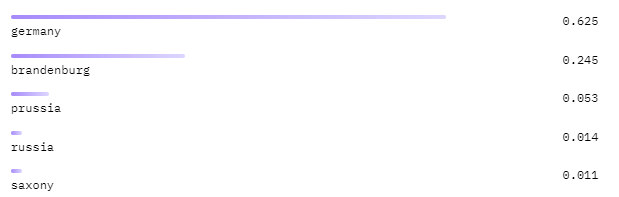
\includegraphics[scale=0.9]{fig/bert_masking_example.png}
  \caption{Example for masking of language models (in this case bert-base-uncased) \cite{bertbaseuncased}, accessed 20-October-2023. The figure shows the 5 most likely words and their corresponding probabilities for the [MASK] token in the sentence above.}%
  \label{fig:bert_masking_example}
\end{figure}

We will present another example (see figure \ref{fig:bert_masking_example2}), showing the capability of language models to also predict linking words since this will be the main focus of this work.

\begin{figure}[H]
  \begin{center}
	\textit{Pizza tastes good}, [MASK] \textit{it's one of the most liked foods in the world}.
  \end{center}
  \centering
  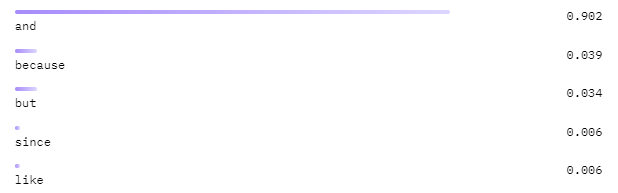
\includegraphics[scale=0.9]{fig/bert_masking_example2.png}
  \caption{Example for linking word masking of language models (in this case bert-base-uncased) \cite{bertbaseuncased}, accessed 20-October-2023. The figure shows the 5 most likely words and their corresponding probabilities for the [MASK] token in the sentence above.}%
  \label{fig:bert_masking_example2}
\end{figure}

The second example shows why we need to use bidirectional models instead of autoregressive models like GPT-3 since the linking word is dependent of both its left and right context. \\
LMs are often times pre-trained on large unlabeled text corpora to generate language representations like word vector embeddings which can later be fine-tuned on more specific tasks. In the next sections, we will present two models that we are going to use.


\subsubsection{BERT}
BERT (Bidirectional Encoder Representations from Transformers) is a LM proposed by Devlin et al. \cite{bert}. Unlike older language models based on LSTMs which can only predict the next token based on the previous tokens, BERT uses a bidirectional approach. This is done by using the aforementioned masked LM pre-training objective. In this approach, a part of the input words gets masked and the training objective is to predict the original word based on its left and right context. Together with the next sentence prediction objective, this completes the pre-training for BERT. This model can now be used to solve many downstream tasks like classification or question answering, just by adding another layer on top, depending on the specific task. BERT set new state-of-the-art performances for many NLP tasks and revolutionized the classic NLP pipeline due to it representing all the steps of the pipeline in one model \cite{bertexplain}.  \\
We will primarily use BERT for masked language modeling and directly for validity and stance classification. There are different types of BERT one can consider, differing for example in the number of parameters, language or case sensitivity. The exact configurations and models used, will be explained in detail in the chapter about implementation. \\

\textbf{Model Architecture} \\
Although we do not need to understand BERT in every detail, one important part is needed in the course of this thesis, namely how the input and output is represented. \\
Most importantly, for every input sequence, a special [CLS] token will be added as first character. This token is used in the last hidden state as an aggregate representation for the entire sequence. It can then be used for further downstream tasks like classification. The vector representations for all the other tokens in the output sequence are only used for token-level tasks like part-of-speech-tagging. Furthermore, a [SEP] token is added after each input sequence. With this technique, we can input two sequences as one into BERT which is used to perform the next sentence prediction task in the pre-training \cite{bert}.


\subsubsection{RoBERTa}
RoBERTa is a LLM that has the same architecture as BERT \cite{roberta}. It improves BERT by
\begin{enumerate}
	\item longer training with more data,
	\item removing the next sentence prediction objective,
	\item training on longer sequences,
	\item dynamically changing the masking pattern.
\end{enumerate}
We are going to use RoBERTa as well since it is commonly used in the approaches described in \cite{argsvalidnovel2022}.

\subsection{Gradient-Boosted Trees}
To classify embeddings which will be created by our linking word probabilities, we are going to primarily use two different ways. The first one is a simple neural network as it is used as additional layer for BERT in a classification setting. The other one will be a Gradient-Boosted Tree. Besides its competitive classification performance, it can also be used to calculate the importance of used features. We will use this technique later on to increase training speed and make the model less vulnerable for overfitting by removing unimportant features. We decided not to use SHAP values \cite{shap} for feature importance simply due to simplicity. \\
Gradient-Boosted Trees are a form of random forests. Both combine multiple decision trees to produce one classifier but they differ in building the individual trees and in combining them \cite{gradboost}. A decision tree splits the data at each node until the leaf nodes are reached. These leaf nodes nodes then correspond to a certain label. In gradient boosting, decision trees with only a few splits are constructed. These trees are then added together sequentially while minimizing a loss function when adding each tree.

\subsubsection{LightGBM}
LightGBM is a gradient boosting frameworks using decision trees which significantly improve the performance and training speed of standard gradient boosting algorithms \cite{lgbm}.

\subsection{Evaluation Metrics}
To evaluate our models, we need to define evaluation metrics. There are many different established metrics to use. In this section we will give an overview of the ones we are going to use along this thesis. These definitions are adapted from Hossin and Sulaiman \cite{metrics}.

\subsubsection{Binary Classification Metrics}

\textbf{Confusion Matrix} \\ \\
For binary classification, one can represent the results in a so called \textit{confusion matrix}. The rows of this matrix represent the predicted classes and the columns represent the true classes. The values in the matrix correspond to the four possible outcomes:
\begin{itemize}
	\item[\textbullet] True Positive (TP): Correctly classified positive instances
	\item[\textbullet] True Negative (TN): Correctly classified negative instances
	\item[\textbullet] False Positive (FP): Wrongly classified negative instances
	\item[\textbullet] False Negative (FN): Wrongly classified positive instances
\end{itemize}
An example of the final matrix is shown in Figure \ref{fig:confusion-matrix}.
\begin{figure}[h]
  \centering
  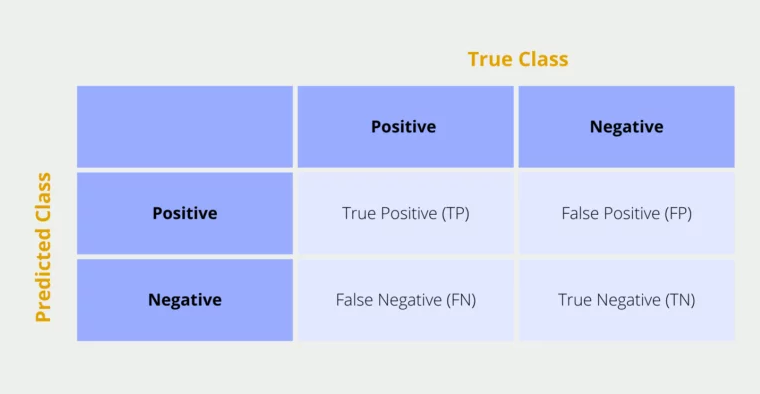
\includegraphics[width=8cm]{fig/confusion_matrix.png}
  \caption{Confusion Matrix \cite{confusion}.}%
  \label{fig:confusion-matrix}
\end{figure}

\textbf{Recall} \\ \\
Recall measures the fraction of positive instances that are correctly classified.

\begin{equation}
	R = \frac{TP}{TP + FN}
\end{equation}

\textbf{Precision} \\ \\
Precision measures the correctly classified positive instances in relation to the overall number of positively predicted instances

\begin{equation}
	P = \frac{TP}{TP + FP}
\end{equation}

\textbf{F1-Score} \\ \\
The F1 score is the harmonic mean between recall and precision.

\begin{equation}
	\text{F1} = \frac{2 \cdot P \cdot R}{P + R}
\end{equation}

To evaluate our models, we will only use the F1-Score to give a good comparison to similar works like the Validity and Novelty Prediction Shared Task \cite{argsvalnov2022}.